\subsection{Campaña experimental y comparación de métodos}

La campaña se diseñó como una comparación pareada. Cada método se evalúa sobre los mismos
mundos, con las mismas cargas, posiciones iniciales, obstáculos, eventos y perfiles de
comunicación. Esta decisión reduce varianza artificial: si un método mejora, la mejora no
procede de haber visto un entorno más fácil. Las métricas se agrupan en cinco bloques:
completitud, factibilidad física, seguridad, recurso y coste computacional. Ningún bloque
sustituye a los demás. Una solución con alta completitud pero colisiones frecuentes no se
acepta como solución de transporte; una solución segura que no mueve la carga tampoco.

\begin{table}[H]
\centering
\scriptsize
\begin{tabularx}{\textwidth}{@{}p{0.22\textwidth}p{0.22\textwidth}X@{}}
\toprule
Familia evaluada & Papel en la comparación & Qué pone a prueba \\
\midrule
Greedy y reglas locales & Baseline mínimo de coste bajo. & Si la distancia y la prioridad local bastan para cerrar coaliciones. \\
Hungarian y referencias centralizadas & Cota de asignación o control con información agregada. & La pérdida por descentralizar y el coste de escalar. \\
CBBA, subastas y variantes de mercado & Baseline distribuido con pujas y consenso. & Si una señal económica escalar soporta cargas físicas. \\
Replicator, Smith y logit & Dinámicas poblacionales interpretables. & La estabilidad de preferencias bajo escasez y saturación. \\
Modelos aprendidos & Políticas entrenadas o imitadoras de referencia. & Adaptabilidad y coste de entrenamiento frente a reglas explícitas. \\
Smith-QR y extensiones físicas & Propuesta principal y variantes. & Cierre entero, capacidad efectiva, wrench, comunicación local y reparación. \\
\bottomrule
\end{tabularx}
\caption{Familias de métodos usadas como contraste experimental.}
\label{tab:familias-metodos-exp}
\end{table}

La lectura estadística se apoya en diferencias pareadas e intervalos de confianza. Cuando
la hipótesis es direccional, se contrasta el método propuesto frente a un comparador
concreto; cuando la pregunta es de familia, se usa una prueba global para decidir si hay
diferencias sistemáticas entre métodos. La tabla siguiente resume la regla de lectura
aplicada a cada bloque de métricas.

\begin{table}[H]
\centering
\scriptsize
\begin{tabularx}{\textwidth}{@{}p{0.18\textwidth}p{0.22\textwidth}X@{}}
\toprule
Bloque & Métrica típica & Criterio de lectura \\
\midrule
Completitud & tasa de cargas servidas, llegada, tareas completadas & Se maximiza, salvo que se logre sacrificando seguridad o factibilidad. \\
Capacidad física & déficit de capacidad, residual wrench, saturación & Se minimiza el déficit; se rechazan falsos positivos físicos. \\
Seguridad & colisiones, despeje, intersección con obstáculo, timeout & Una mejora de tiempo no compensa una degradación de seguridad. \\
Recurso & energía, distancia, mensajes, memoria & Sirve para diferenciar métodos con éxito similar. \\
Cómputo & tiempo de cálculo y escalado con $N$ & Una referencia centralizada deja de ser operativa cuando excede tiempo o memoria. \\
\bottomrule
\end{tabularx}
\caption{Bloques de métricas y decisión experimental.}
\label{tab:bloques-metricas-exp}
\end{table}

\subsubsection{SP1: reclutamiento de coaliciones}

SP1 mide si una regla consigue reunir suficientes robots alrededor de cargas heterogéneas
antes de introducir capacidad continua o wrench. La referencia centralizada y su replay
alcanzan una tasa de carga servida de $0{,}8469$. El método aprendido con decodificador de
quórum alcanza $0{,}8463$, con una brecha media frente a la referencia de $0{,}0043$. La
diferencia frente a greedy, Hungarian y CBBA es clara en completitud, aunque el coste de
inferencia es mayor que el de las reglas clásicas. Smith cardinality queda en $0{,}5590$:
la presión poblacional por sí sola no cierra quórums enteros de forma competitiva.

\begin{figure}[H]
\centering
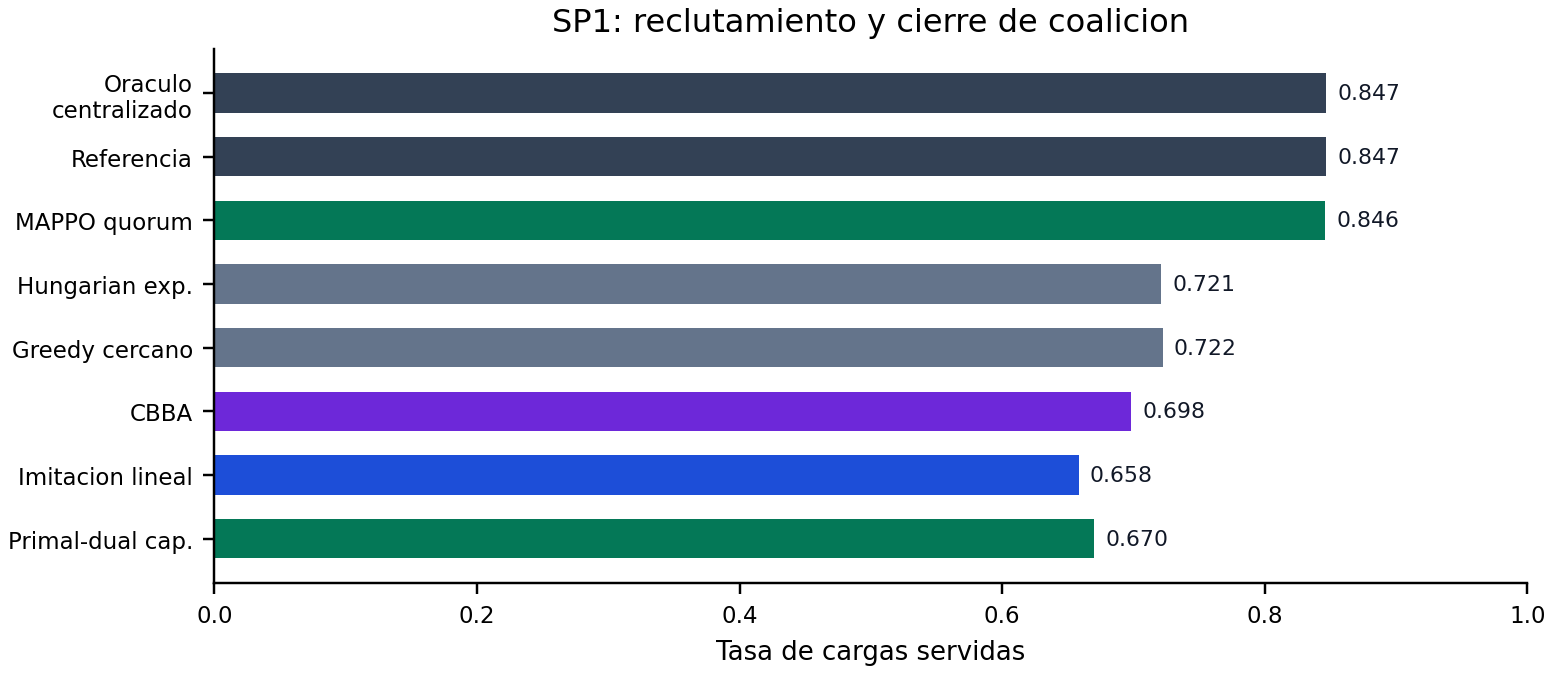
\includegraphics[width=0.92\textwidth]{figures/fig-sp1-primary.png}
\caption{SP1: métrica primaria de reclutamiento por método.}
\label{fig:sp1-primary}
\end{figure}

La lectura Pareto ayuda a no exagerar el resultado. Greedy y Hungarian son muy baratos,
pero pierden demanda servida; CBBA comunica y negocia, pero no supera la limitación de
una utilidad aún demasiado escalar; el método aprendido se aproxima a la referencia, pero
compra esa mejora con entrenamiento y mayor latencia de inferencia. La contribución de
SP1 no es que el aprendizaje gane siempre, sino que demuestra el valor del cierre entero
cuando la tarea exige quorum.

\begin{figure}[H]
\centering
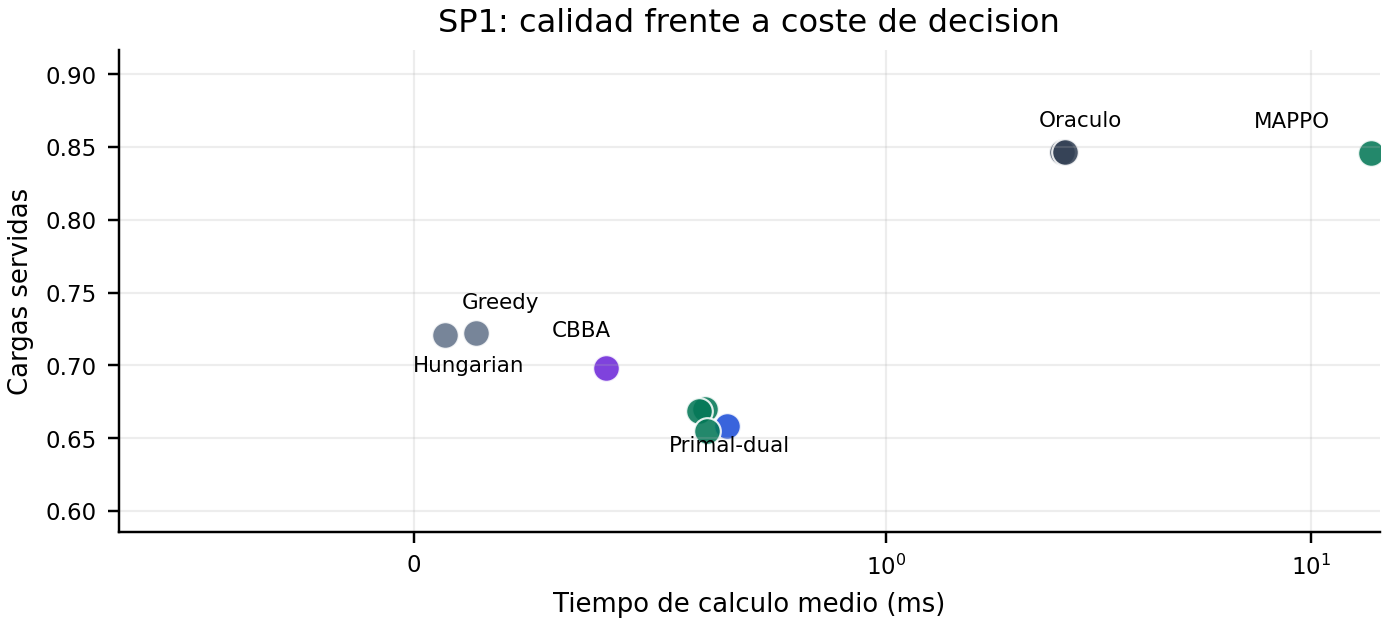
\includegraphics[width=0.86\textwidth]{figures/fig-sp1-pareto.png}
\caption{SP1: compromiso entre calidad de reclutamiento y recurso computacional.}
\label{fig:sp1-pareto}
\end{figure}

El contraste de hipótesis confirma esta lectura. Las diferencias entre métodos en brecha
teórica son significativas, con $W=0{,}6063$ en el contraste global. La comparación
pareada entre el método aprendido y la imitación lineal reduce la brecha media en
$0{,}3731$, y frente a Hungarian reduce $0{,}2722$. La ventaja de Smith puro no está en
completitud, sino en coste: su tiempo es inferior al del método aprendido por más de
$13$ ms de media. En otras palabras, SP1 separa dos propiedades: cerrar bien y cerrar
barato.

\subsubsection{SP2: capacidad efectiva}

SP2 elimina una simplificación cómoda: no todos los robots aportan lo mismo. La referencia
de capacidad alcanza $0{,}4868$ de éxito, mientras que el comparador descentralizado
aprendido con mayor éxito en esta métrica alcanza $0{,}2633$. Greedy capacity queda cerca en completitud
($0{,}2190$), pero con mayor brecha frente a la referencia. El resultado más útil es
negativo para una variante propuesta: primal-dual capacity no supera a greedy en éxito de
capacidad, con $0{,}1000$ frente a $0{,}2190$. La campaña obliga a ajustar el discurso:
la presión marginal mejora la trazabilidad, pero no basta si el score no aproxima bien la
capacidad real de cada coalición.

\begin{figure}[H]
\centering
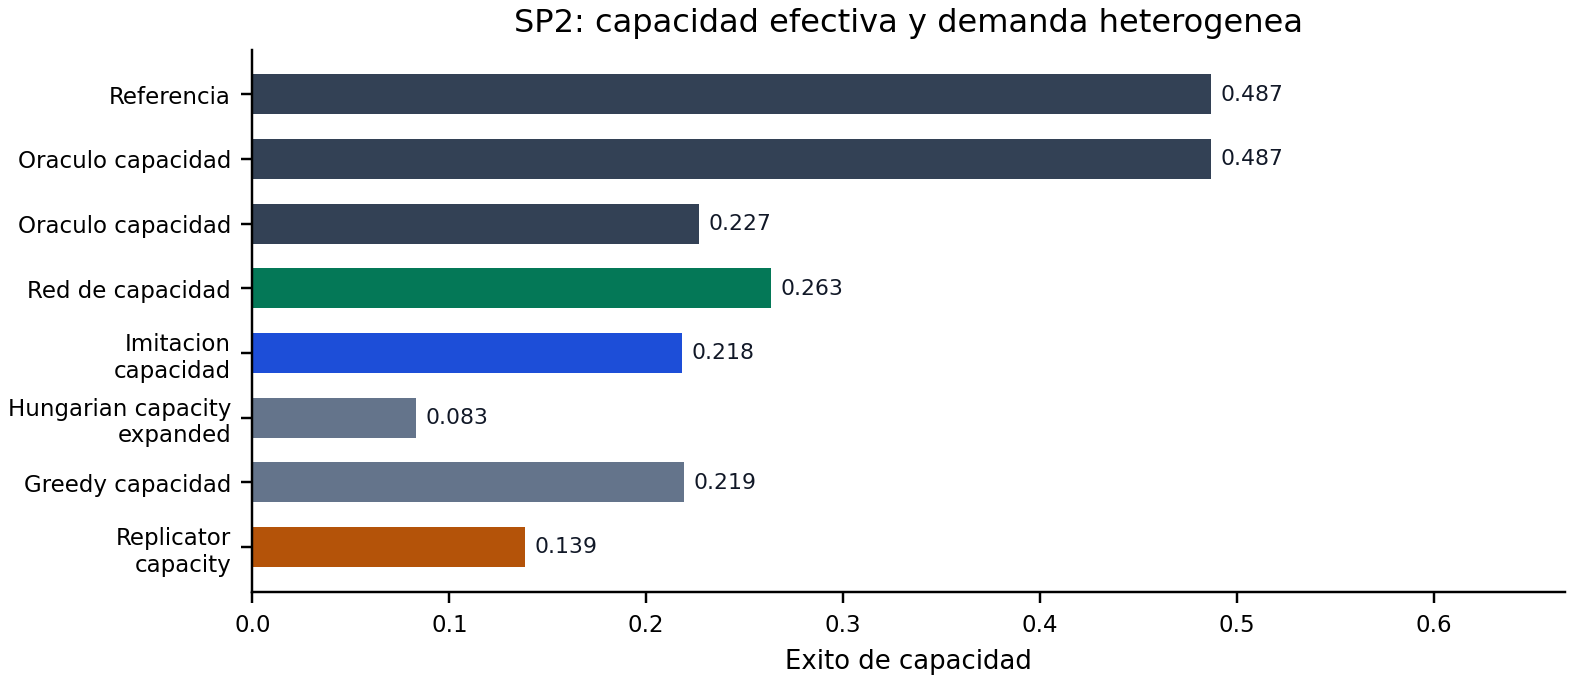
\includegraphics[width=0.92\textwidth]{figures/fig-sp2-primary.png}
\caption{SP2: éxito de capacidad efectiva bajo heterogeneidad de robots y cargas.}
\label{fig:sp2-primary}
\end{figure}

La hipótesis que sí queda soportada es la diferencia entre familias. El contraste global
en brecha de capacidad da $W=0{,}7100$, lo que indica separación fuerte entre métodos.
La política neuronal reduce la brecha frente a la imitación lineal en $0{,}0097$, con
significación tras corrección. La conclusión técnica es sobria: al introducir capacidad
efectiva, la cardinalidad deja de ser un proxy fiable; los métodos que usan señales de
capacidad ganan información, pero deben calibrarse con cuidado para no sobrepenalizar
coaliciones útiles o sobrerrecompensar capacidad nominal.

\subsubsection{SP3: factibilidad wrench}

SP3 es el primer punto donde la tesis abandona una evaluación escalar. Todos los métodos
pueden alcanzar una tasa de factibilidad wrench aparente de $0{,}5$ en el agregado porque
la campaña contiene casos factibles e inviables balanceados. La diferencia aparece en los
falsos positivos. La referencia wrench mantiene tasa $0$, mientras que la asignación
escalar acepta indebidamente la mitad de los casos. CBBA slots reduce los falsos positivos
a $0{,}1632$; Smith-QR wrench marginal queda cerca de $0{,}4830$, lo que muestra que una
señal marginal no sustituye a una verificación explícita de contactos.

\begin{figure}[H]
\centering
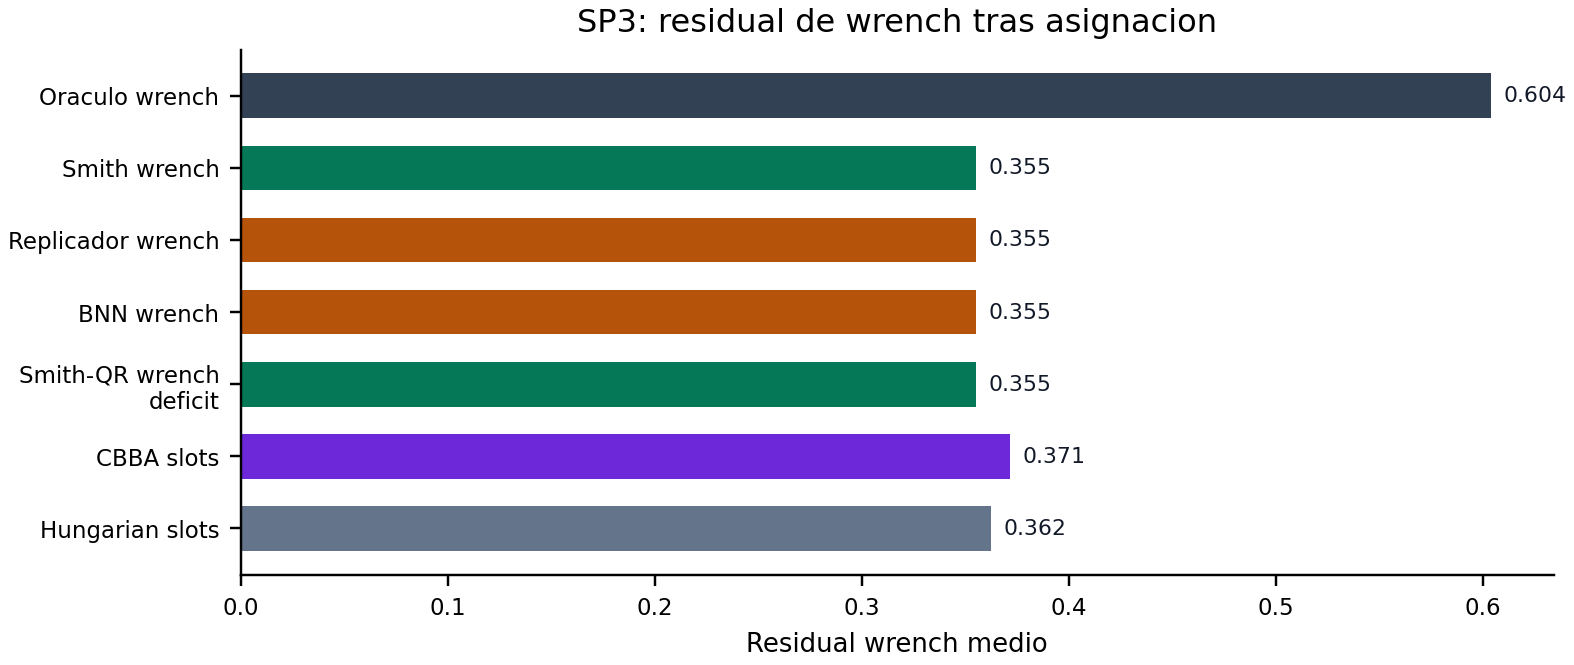
\includegraphics[width=0.92\textwidth]{figures/fig-sp3-residual.png}
\caption{SP3: residual de fuerza y torque por método.}
\label{fig:sp3-residual}
\end{figure}

\begin{figure}[H]
\centering
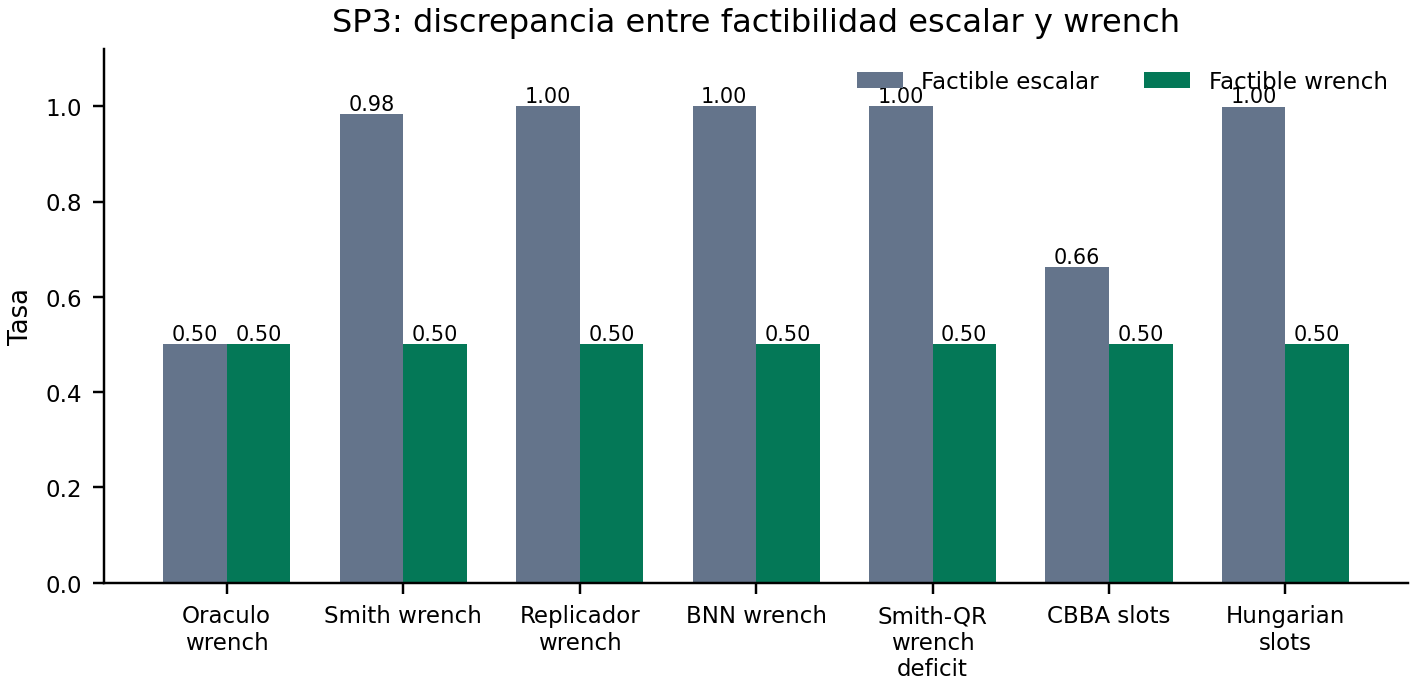
\includegraphics[width=0.92\textwidth]{figures/fig-sp3-scalar-wrench.png}
\caption{SP3: comparación entre éxito escalar y éxito wrench.}
\label{fig:sp3-scalar-wrench}
\end{figure}

El contraste específico sobre cargas rotacionales confirma el fallo del criterio escalar:
la tasa de falsos positivos frente a referencia es $0{,}5000$, con intervalo
$[0{,}4790,\ 0{,}5225]$. La lección es directa. Un método puede asignar robots a una
carga y declarar cobertura, pero esa cobertura no vale si los contactos no generan el
par necesario. Esta es la razón por la que el TFM trata el wrench como puerta de
factibilidad, no como métrica secundaria.

\subsubsection{SP4: movimiento seguro}

SP4 introduce trayectorias, obstáculos y coste de llegada. El ranking por score favorece
reglas rápidas como APF o direct-to-target porque no sufren timeout y resuelven pronto,
pero su tasa de colisión queda alrededor del $4{,}7$--$5{,}0\%$. Las referencias con CBF
reducen la colisión a torno al $1{,}0$--$1{,}2\%$, a cambio de timeout cercano al
$8\%$. Smith-QR motion y primal-dual motion se acercan al régimen seguro, con colisión
alrededor de $1{,}2\%$, aunque pagan más timeout que las reglas directas.

\begin{figure}[H]
\centering
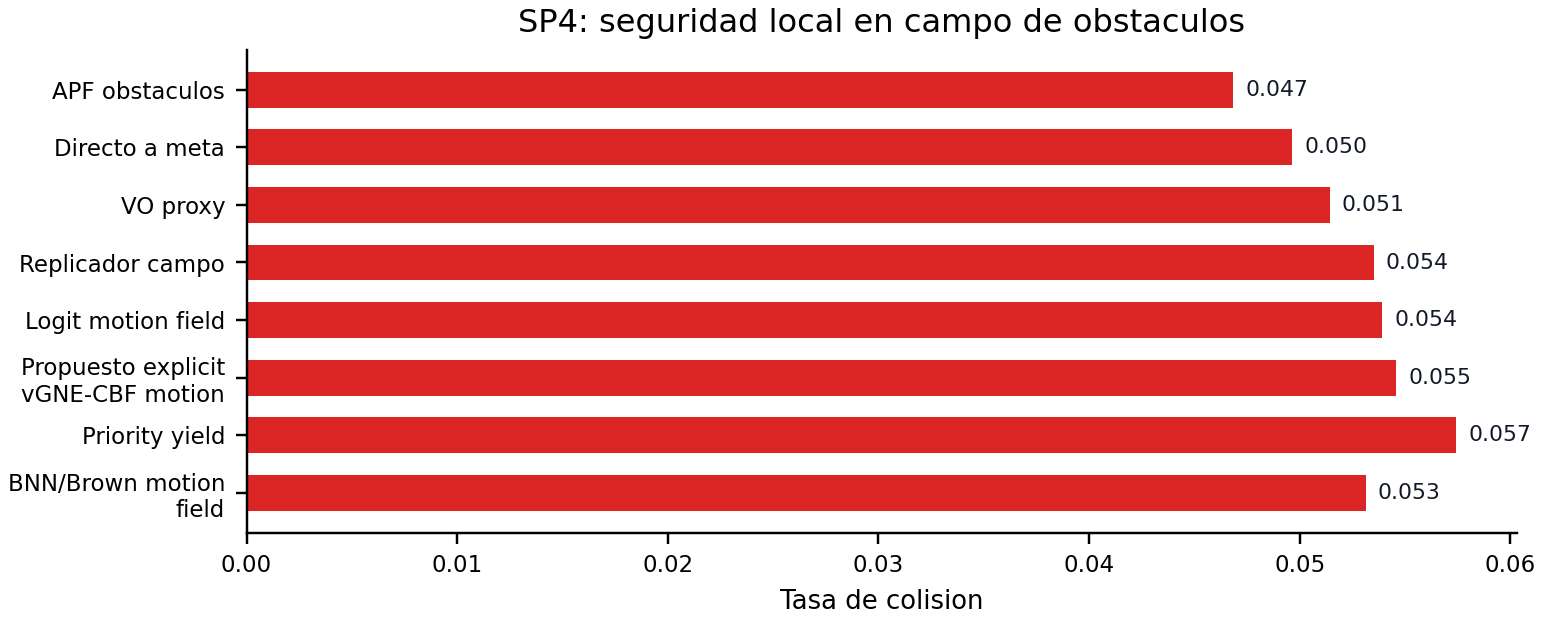
\includegraphics[width=0.78\textwidth]{figures/fig-sp4-collision-scenario.png}
\caption{SP4: tasa de colisión por escenario y familia de movimiento.}
\label{fig:sp4-collision-scenario}
\end{figure}

\begin{figure}[H]
\centering
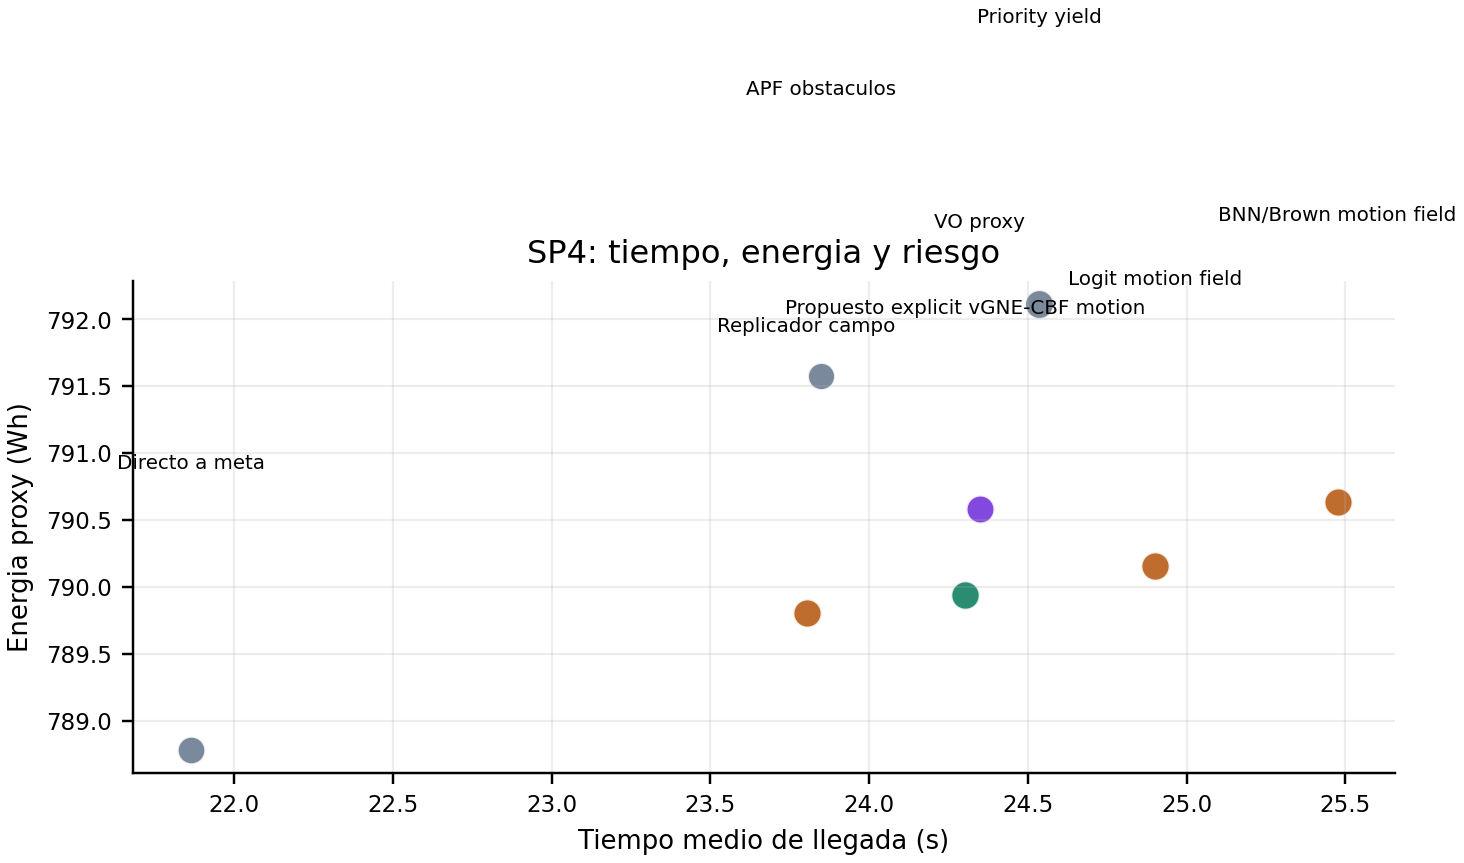
\includegraphics[width=0.78\textwidth]{figures/fig-sp4-time-energy.png}
\caption{SP4: compromiso entre tiempo, energía y seguridad.}
\label{fig:sp4-time-energy}
\end{figure}

Las hipótesis de seguridad son claras. La referencia CBF reduce la colisión frente a
direct-to-target en $0{,}0392$, y el filtro CBF lo hace en $0{,}0381$. El método tensor
también reduce colisión frente a la regla directa en $0{,}0374$. En cambio, la hipótesis
de ahorro energético de Smith frente a CBF no queda soportada. Esta combinación evita una
lectura simplista: los métodos con barrera son mejores en seguridad, pero no ganan gratis
en tiempo ni energía. SP4 define el punto de equilibrio que luego SP5 hereda con la carga
extendida.

\subsubsection{SP5: transporte de carga extendida}

SP5 desplaza la métrica desde el robot hacia el objeto. Las variantes cargo alcanzan
llegada del $100\%$; las variantes de empuje sin modelo suficiente de carga quedan en
$0\%$ o muy cerca de cero. La referencia centralizada obtiene score $300{,}73$ y
formación rota $0{,}0161$. La variante Hamiltoniana propuesta alcanza score
$297{,}32$, llegada $1{,}0$, cero colisiones y menor energía que la referencia
($751{,}97$ frente a $896{,}06$ Wh), aunque con formación rota $0{,}0555$. La lectura
correcta es de compromiso: la propuesta ejecuta el transporte y reduce energía, pero no
mejora la integridad de formación frente a las mejores referencias.

\begin{figure}[H]
\centering
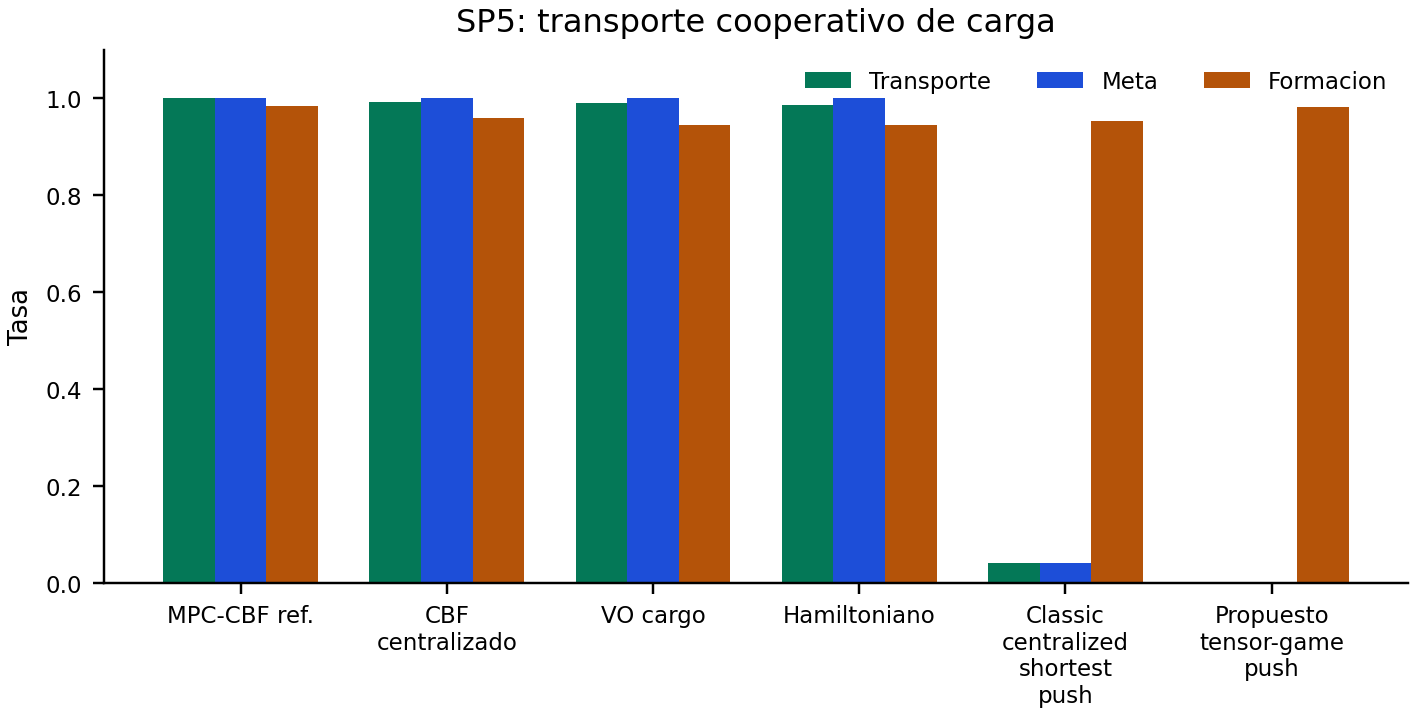
\includegraphics[width=0.92\textwidth]{figures/fig-sp5-primary.png}
\caption{SP5: score de transporte cooperativo de carga extendida.}
\label{fig:sp5-primary}
\end{figure}

El contraste estadístico separa con fuerza las variantes cargo de las variantes push. La
referencia reduce la brecha frente a APF push en $1{,}0$, y el contraste global de score
da $W=0{,}7313$. En cambio, la hipótesis de que la variante Hamiltoniana reduzca ruptura
de formación frente a VO cargo no queda soportada. Este resultado negativo es útil: la
formulación port-Hamiltoniana aporta coherencia energética y transporte de la carga, pero
no sustituye a una capa de formación más estricta cuando el objetivo es mantener slots
con error mínimo.

\subsubsection{SP6: recuperación ante eventos}

SP6 mide reparación bajo fallos de robot, batería, información retardada y cargas
inviables. La recuperación guarded wrench-market obtiene el mayor score agregado
($144{,}84$), con tasa de completitud $0{,}7163$ y cero colisiones. La referencia
centralizada queda en $0{,}7115$ de completitud. Primal-dual, tensor-flow y Smith-QR
se mantienen cerca, todos entre $0{,}706$ y $0{,}709$. La distancia con greedy y CBBA
no es enorme en completitud, pero sí en brecha frente a referencia y carga perdida.

\begin{figure}[H]
\centering
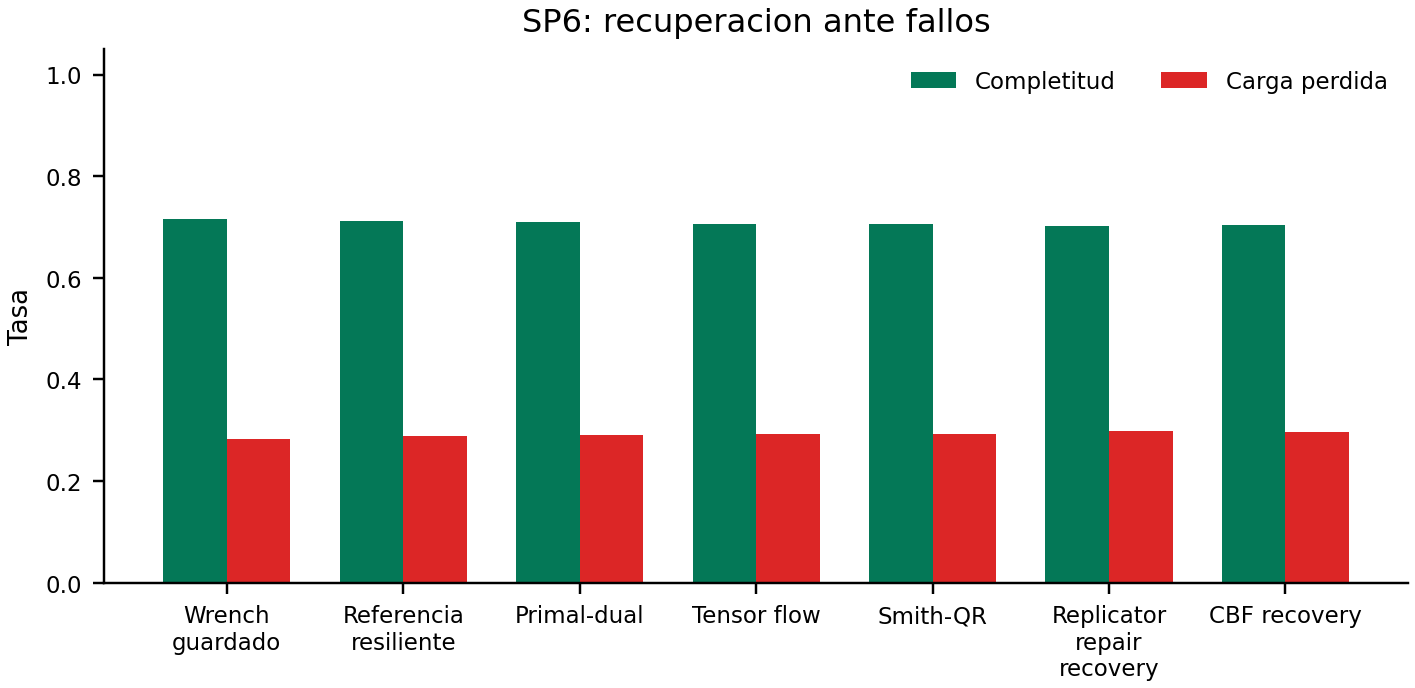
\includegraphics[width=0.92\textwidth]{figures/fig-sp6-primary.png}
\caption{SP6: rendimiento agregado ante recuperación, fallo y reasignación.}
\label{fig:sp6-primary}
\end{figure}

La hipótesis principal de pérdida de carga sí queda soportada: guarded wrench-market
reduce la tasa de carga perdida frente a greedy descentralizado en $0{,}0248$. También
reduce la brecha frente a CBBA en $0{,}0684$. No queda soportada, en cambio, una mejora
clara de completitud frente a Smith-QR. Esto perfila mejor la contribución: el valor de la
guardia wrench-market no está en ganar todas las tareas, sino en evitar reparaciones
físicamente incoherentes y reducir pérdidas cuando el evento rompe la coalición inicial.

\subsubsection{SP7: comunicación y sensado degradado}

SP7 fuerza al sistema a operar con información incompleta. La variante connectivity-aware
wrench game obtiene el mejor score ($14{,}55$), llegada $0{,}1615$ y formación rota
$0{,}1164$. El controlador centralizado de comunicación completa queda por debajo
($-35{,}15$), con llegada $0{,}1462$ y formación rota $0{,}4092$. La diferencia no se
debe a magia descentralizada, sino a una señal que penaliza conectividad frágil y repara
coaliciones cuando la información llega tarde.

\begin{figure}[H]
\centering
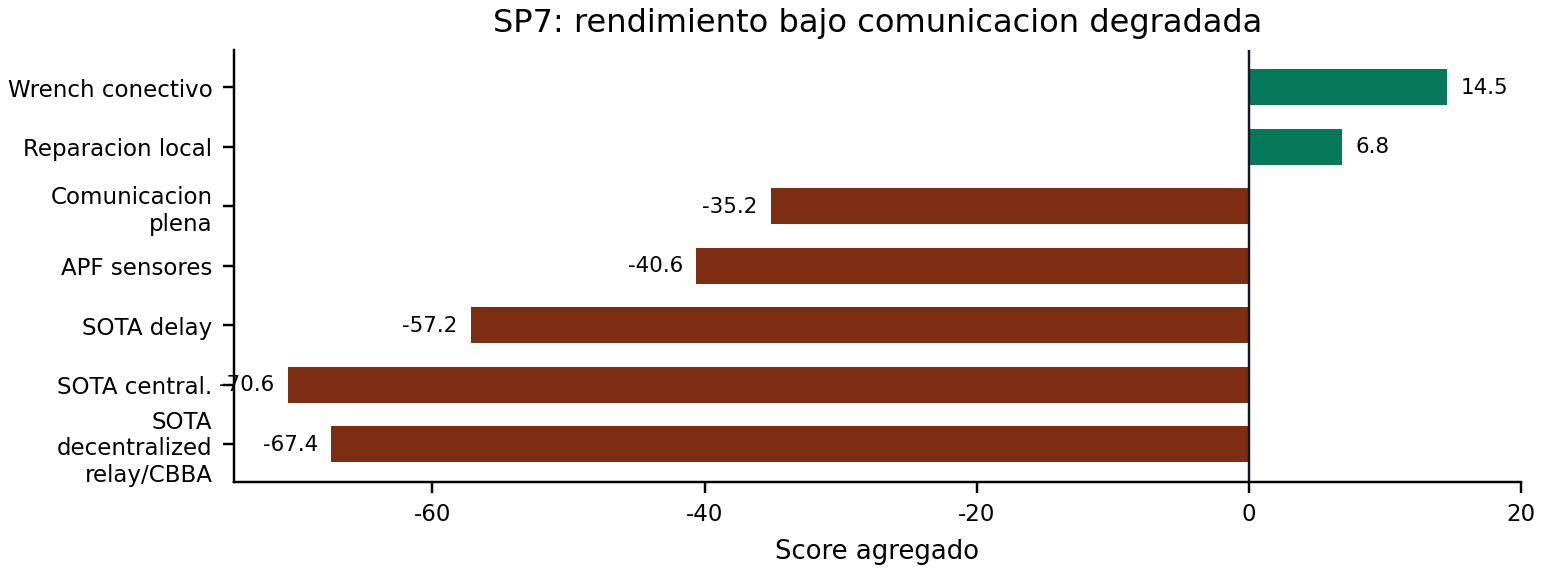
\includegraphics[width=0.92\textwidth]{figures/fig-sp7-primary.png}
\caption{SP7: rendimiento bajo degradación de comunicación y sensado.}
\label{fig:sp7-primary}
\end{figure}

El radio de comunicación muestra asociación positiva con la conectividad de coalición,
con $\rho=0{,}8863$. En perfiles duros, la variante propuesta mejora el score de red
frente al control centralizado clásico en $0{,}2122$, con tamaño de efecto alto. El
contraste global bajo comunicación intermitente no detecta diferencias entre todos los
métodos, lo que también importa: cuando el canal cae demasiado, la arquitectura solo
puede recuperar hasta donde el grafo temporal permite observar la carga y los compañeros.

\subsubsection{SP8: escalabilidad de flota}

SP8 mide la frontera de practicidad al crecer la flota hasta escalas de almacén. Las tres
mejores variantes propuestas mantienen solved rate $1{,}0$ y completitud entre
$0{,}1561$ y $0{,}1618$. Classic local greedy y auction market local quedan alrededor de
$0{,}061$, mientras que Hungarian expandido cae a $0{,}0187$ con timeout $0{,}6$ y la
referencia de coalición a $0{,}0325$ con timeout $0{,}8$. La memoria media estimada de
las variantes distribuidas se mantiene alrededor de $2{,}08$ MB, frente a más de
$1254$ MB en referencias centralizadas.

\begin{figure}[H]
\centering
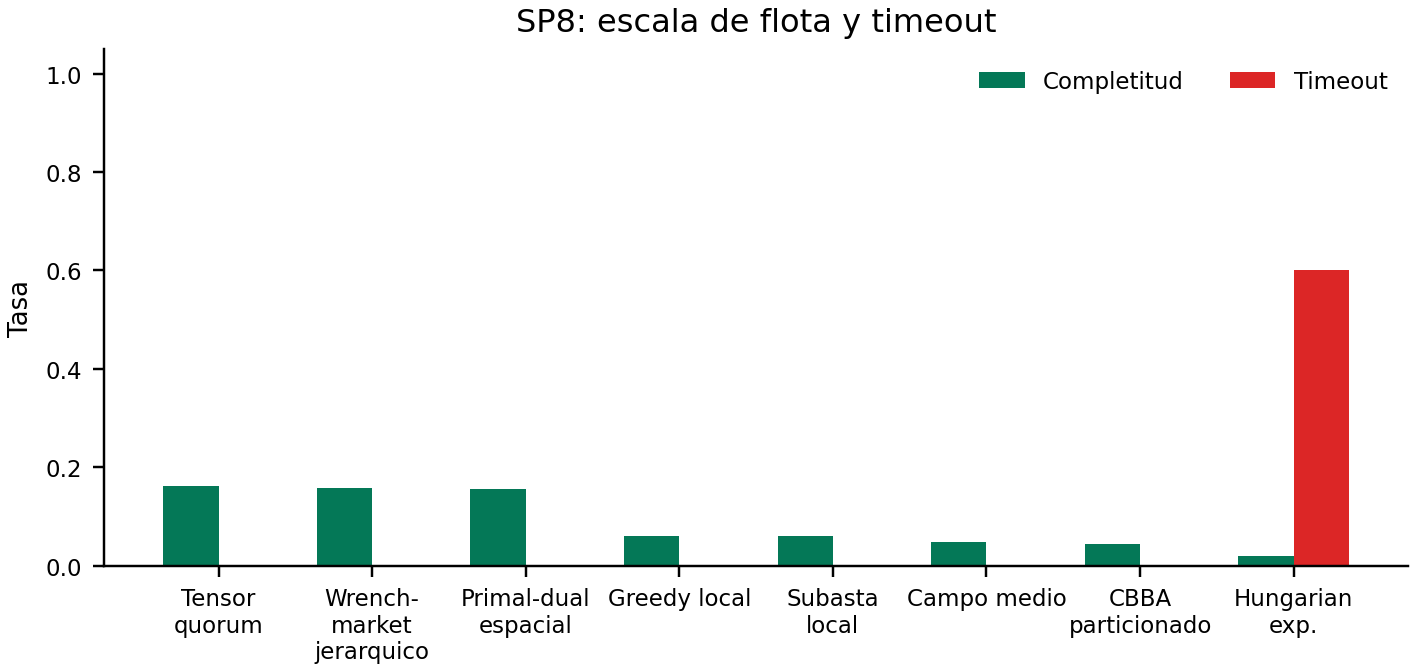
\includegraphics[width=0.92\textwidth]{figures/fig-sp8-primary.png}
\caption{SP8: métrica primaria de escala en flotas grandes.}
\label{fig:sp8-primary}
\end{figure}

\begin{figure}[H]
\centering
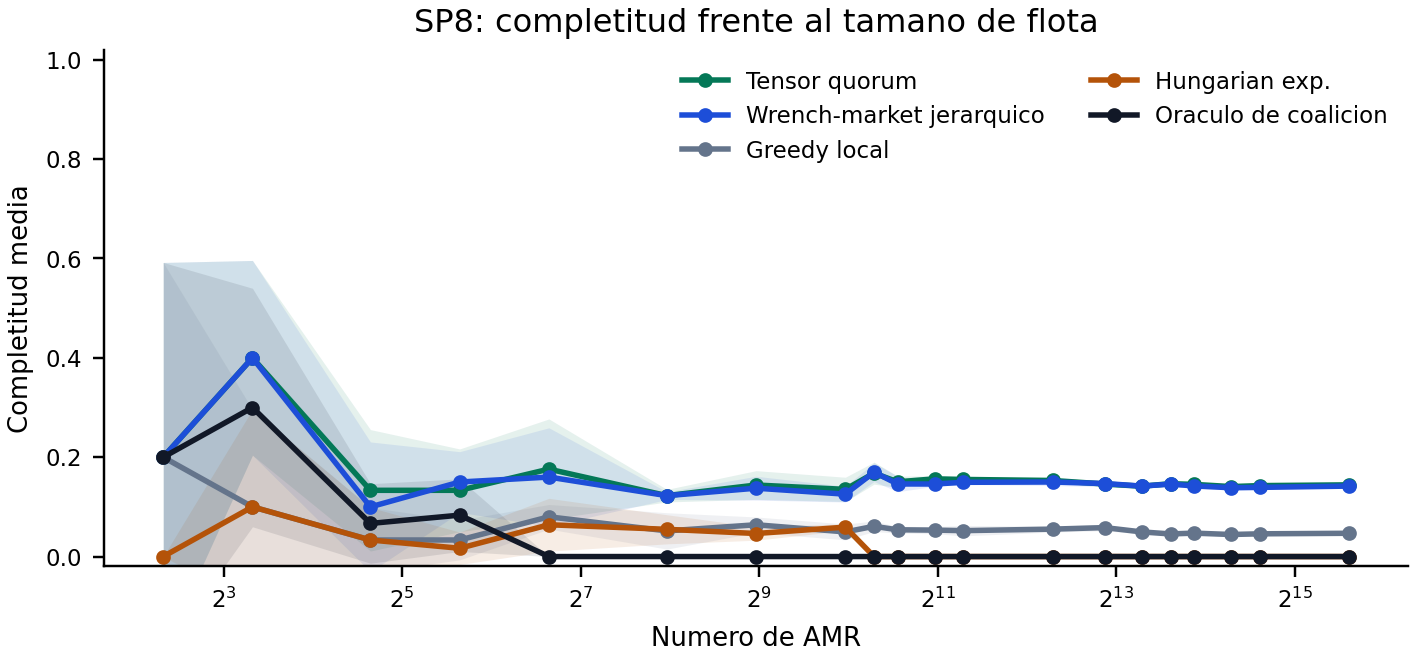
\includegraphics[width=0.92\textwidth]{figures/fig-sp8-scale-ci.png}
\caption{SP8: evolución de completitud con el tamaño de flota.}
\label{fig:sp8-scale-ci}
\end{figure}

La hipótesis de escala queda soportada por tres resultados. Primero, el timeout de la
referencia centralizada aumenta con la escala, con $\rho=0{,}6937$. Segundo, la variante
jerárquica mejora la completitud frente a greedy local en $0{,}0964$. Tercero, la misma
variante mejora la factibilidad wrench frente a Hungarian expandido en $0{,}1741$. La
lectura industrial es prudente: SP8 no demuestra despliegue real, pero sí muestra que las
familias distribuidas y jerárquicas conservan una relación calidad-recurso más defendible
cuando la enumeración centralizada deja de ser viable.

\subsubsection{Tabla transversal de resultados}

\begin{table}[H]
\centering
\scriptsize
\begin{tabularx}{\textwidth}{@{}p{0.06\textwidth}p{0.22\textwidth}p{0.24\textwidth}X@{}}
\toprule
SP & Mejor lectura favorable & Comparador crítico & Límite que queda abierto \\
\midrule
SP1 & MAPPO con decodificador alcanza $0{,}8463$ de cargas servidas, casi igual que la referencia. & Smith cardinality queda en $0{,}5590$. & El cierre entero pesa más que la presión continua pura. \\
SP2 & La política neuronal mejora a la imitación lineal y supera a greedy en score. & La referencia de capacidad sigue en $0{,}4868$ de éxito. & La capacidad efectiva requiere calibración más fina que la cardinalidad. \\
SP3 & La referencia wrench elimina falsos positivos; CBBA slots reduce parte del error escalar. & La asignación escalar acepta el $50\%$ de casos inválidos. & Smith-QR necesita verificación explícita de contacto para no aceptar torque falso. \\
SP4 & CBF y campos con barrera reducen colisiones frente a direct-to-target. & Los métodos rápidos ganan score cuando el timeout pesa más que la colisión. & Seguridad y tiempo siguen en tensión. \\
SP5 & Hamiltonian cargo llega al $100\%$ y reduce energía frente a la referencia. & La referencia conserva mejor integridad de formación. & Falta endurecer el control de slots sin perder eficiencia. \\
SP6 & Guarded wrench-market reduce carga perdida y brecha frente a CBBA. & La mejora frente a Smith-QR en completitud no es concluyente. & La recuperación gana por evitar fallos graves, no por dominar todas las tareas. \\
SP7 & Connectivity-aware wrench game mejora bajo perfiles duros y reduce ruptura de formación. & La intermitencia extrema borra diferencias globales. & La conectividad temporal impone un límite físico a la información disponible. \\
SP8 & Tensor quorum y wrench-market jerárquico superan a greedy y referencias centralizadas en escala. & Las referencias centralizadas sufren timeout y memoria alta. & La validación sigue siendo mesoscópica, no industrial directa. \\
\bottomrule
\end{tabularx}
\caption{Lectura transversal de resultados, comparadores y límites.}
\label{tab:lectura-transversal-resultados}
\end{table}

\subsubsection{Comparación por familia}

Los métodos clásicos siguen siendo necesarios. Greedy y APF dan tiempos bajos y una línea
base honesta. Hungarian y CBF centralizados fijan cotas, aunque pierden practicidad al
crecer $N$ o al requerir información agregada. CBBA y subastas son competitivos cuando
la utilidad cabe en una puja local; su debilidad aparece cuando la puja debe representar
torque, seguridad de carga o comunicación temporal.

Los métodos aprendidos cumplen una función distinta. En SP1 y SP2 capturan estructura que
las reglas lineales pierden, pero su mejora depende de la distribución de entrenamiento y
no trae por sí sola una garantía física. Por eso la tesis no los usa como argumento de
cierre, sino como contraste moderno: muestran cuánto se puede ganar si se permite
entrenar una política sobre escenarios repetidos.

Las variantes model-based propuestas son más irregulares, pero más explicables. En SP2 no
dominan; en SP3 necesitan un filtro wrench explícito; en SP5 la versión Hamiltoniana
transporta la carga con menor energía pero no reduce al mínimo la ruptura de formación;
en SP6 y SP7 ganan sentido porque las guardias físicas y la conectividad entran en la
decisión; en SP8 recuperan fuerza al crecer la flota, donde la enumeración centralizada
deja de ser razonable.

Esta comparación sostiene la tesis central. No existe un método que gane todo. Existe una
arquitectura que conserva señales físicas locales y permite razonar sobre fallos. Esa
diferencia es académicamente más valiosa que presentar una tabla de victoria universal:
explica dónde la propuesta funciona, dónde no, y qué parte del modelo causa cada cambio.

\subsubsection{Resultados negativos y validez de la inferencia}

La campaña contiene resultados negativos deliberadamente conservados. SP2 no confirma que
primal-dual capacity supere a greedy en éxito de capacidad. SP4 no confirma ahorro
energético de Smith frente a CBF. SP5 no confirma que Hamiltonian cargo reduzca ruptura
de formación frente a VO cargo. SP6 no confirma mejora clara de completitud frente a
Smith-QR. SP7 no detecta diferencia global bajo comunicación intermitente extrema.

Estos resultados no debilitan el trabajo; delimitan la afirmación defendible. El TFM no
presenta Smith-QR como algoritmo universal, sino como una integración físico-económica
que mejora ciertos regímenes: cierre entero de coalición, recuperación con guardias,
comunicación degradada y escala. Donde la evidencia no soporta superioridad, el texto lo
mantiene como límite. Esa disciplina evita confundir simulación con despliegue industrial
y deja una agenda clara: mejor calibración de capacidad, verificación wrench integrada en
tiempo real, control de slots más estricto y validación física con AMR reales.

Los resultados sostienen cuatro conclusiones técnicas. Primero, la abstracción escalar es
insuficiente: una carga puede parecer cubierta y seguir sin torque disponible. Segundo,
la coordinación distribuida necesita mecanismos híbridos; Smith aporta presión
interpretable, pero el quórum entero, la memoria y las guardias físicas son necesarios
para ejecutar. Tercero, los comparadores aprendidos son valiosos como contraste, aunque
su mejora no debe confundirse con garantía estructural ni dominancia global. Cuarto, la
escala favorece arquitecturas que aceptan decisiones locales reparables antes que
optimizaciones globales rígidas.

El principal resultado negativo también es relevante: ninguna familia domina todas las
métricas. Los métodos rápidos pueden perder seguridad; los métodos seguros pueden pagar
tiempo o energía; los métodos aprendidos pueden mejorar en un régimen y fallar fuera de
él; y las referencias centralizadas son útiles como cota, no como solución desplegable
cuando la flota crece. Esta lectura permite defender la memoria como una contribución
metodológica y experimental sólida en simulación.
